\documentclass[11pt,twocolumn]{article}

\usepackage[margin=0.75in]{geometry}
\usepackage{times}
\usepackage{graphicx}
\usepackage{booktabs}
\usepackage{hyperref}
\usepackage{xcolor}
\usepackage{amsmath}
\usepackage{amssymb}
\usepackage{float}
\usepackage{enumitem}
\usepackage{fancyhdr}
\usepackage{titlesec}
\usepackage{caption}
\usepackage{array}
\usepackage{tabularx}
\usepackage{listings}
\usepackage{tikz}
\usepackage{pgfplots}
\pgfplotsset{compat=1.18}
\usetikzlibrary{positioning,arrows.meta,shapes.geometric,calc,patterns,fit,decorations.pathreplacing}

\hypersetup{
    colorlinks=false,
    linkcolor=black,
    citecolor=black,
    urlcolor=black,
    pdfborder={0 0 0.5},
    linkbordercolor={0.5 0.5 0.5},
    citebordercolor={0.5 0.5 0.5},
    urlbordercolor={0.5 0.5 0.5},
}

\captionsetup{font=small,labelfont=bf}

\titleformat{\section}{\large\bfseries}{\thesection.}{0.5em}{}
\titleformat{\subsection}{\normalsize\bfseries}{\thesubsection}{0.5em}{}

\pagestyle{fancy}
\fancyhf{}
\fancyfoot[C]{\thepage}
\renewcommand{\headrulewidth}{0pt}

\lstset{
    basicstyle=\ttfamily\scriptsize,
    breaklines=true,
    breakatwhitespace=false,
    columns=fullflexible,
    keepspaces=true,
    frame=single,
    framesep=2pt,
    xleftmargin=3pt,
    xrightmargin=3pt,
    aboveskip=6pt,
    belowskip=6pt,
    backgroundcolor=\color{gray!8},
    rulecolor=\color{gray!40},
}

\title{\Large\textbf{Re-enabling Fused-Off Compute Units\\on the AMD BC-250 APU\\via Register-Level Modification}}

\author{
Scott Duggan\\
\textit{Independent Research}\\
\texttt{duggasco@gmail.com}
}

\date{May 2026}

\begin{document}

\twocolumn[
\maketitle
\begin{abstract}
\noindent The AMD BC-250 is a standalone single-board computer built around a salvaged PlayStation~5 APU (``Ariel''), shipping with 24 of 40 physical RDNA~2 GPU compute units (CUs) active. Industry consensus holds that CU harvesting on modern AMD silicon is enforced by irreversible hardware fuses, rendering disabled CUs permanently inaccessible. We demonstrate that this assumption is incorrect for the BC-250: the CU disable mask resides in a software-writable configuration register (\texttt{CC\_GC\_SHADER\_ARRAY\_CONFIG}), and a second power-gating register (\texttt{SPI\_PG\_ENABLE\_STATIC\_WGP\_MASK}) gates hardware dispatch. By writing both registers from within the kernel GPU driver's initialization path, we re-enabled all 40~CUs, achieving a 1.54$\times$ improvement in LLM inference prefill throughput (302 to 466~tok/s) with zero compute errors across extensive stress testing. The technique has been verified on three separate boards, and the patch is publicly available~\cite{unlock}. To our knowledge, this is the first documented instance of CU re-enablement on a production AMD APU through software-only means.
\end{abstract}
\vspace{1em}
]

\section{Introduction}

\subsection{Background}

Semiconductor yield management routinely produces dies where a subset of functional units fail quality or power targets. Rather than discard these dies, manufacturers \textit{harvest} (disable) the failing units and sell the part as a lower-tier SKU. This practice is well-documented across AMD, NVIDIA, and Intel product lines and is a key economic lever in modern chip manufacturing.

The AMD BC-250 represents an unusual case. Originally fabricated as a full Navi~10 die---the same 7nm TSMC silicon used in the Radeon RX~5700~XT and PlayStation~5---these APUs were binned out of Sony's PS5 qualification process. AMD repurposed them for cryptocurrency mining by pairing the die with 6 active Zen~2 CPU cores, 16~GB of unified GDDR6 memory, and a minimal standalone PCB manufactured by ASRock Rack. The result is a complete single-board computer requiring no host system, available on the secondary market for \$50--150.

Each BC-250 ships with 24 of 40 GPU CUs active (40\% harvested), organized as 6 active CUs per shader array across 4 shader arrays. With the mining market's collapse, these boards have found a second life as ultra-low-cost AI inference nodes, where GPU CU count directly constrains throughput. An active community of over 3,500 members has developed custom BIOS firmware, GPU power governors, cooling solutions, and software tooling to support this use case.

\subsection{Prior Assumptions}

The prevailing model for AMD CU harvesting holds that:

\begin{enumerate}[nosep]
    \item On-die fuses are blown during manufacturing to permanently disable defective or surplus CUs.
    \item The Platform Security Processor (PSP) reads these fuses during early boot and programs the GPU's configuration registers accordingly.
    \item The resulting CU mask is a read-only hardware constant that the OS driver can only observe, never modify.
    \item \texttt{GC\_USER\_SHADER\_ARRAY\_CONFIG} allows software to disable \textit{additional} CUs but cannot re-enable fuse-disabled ones, since the effective mask is the logical OR of the hardware and user masks.
\end{enumerate}

Our work challenges assumptions 2, 3, and 4.

\subsection{Contribution}

We present:
\begin{itemize}[nosep]
    \item A register-level characterization of the CU harvesting mechanism on the BC-250 APU.
    \item Proof that \texttt{CC\_GC\_SHADER\_ARRAY\_CONFIG} is software-writable from inside the kernel driver.
    \item Discovery of a second required register (\texttt{SPI\_PG\_ENABLE\_STATIC\_WGP\_MASK}) that gates hardware dispatch to re-enabled CUs.
    \item A controlled 4-state experiment isolating each register's contribution.
    \item Performance and stability characterization under real LLM inference workloads.
    \item Verification across three separate boards, all showing identical results.
\end{itemize}

\section{Hardware Platform}

The BC-250 is a unified APU---CPU, GPU, and memory share a single die and a single 16~GB GDDR6 memory pool. Table~\ref{tab:hw} summarizes the key specifications.

\begin{table}[H]
\centering
\caption{BC-250 APU specifications.}
\label{tab:hw}
\small
\begin{tabular}{@{}ll@{}}
\toprule
\textbf{Parameter} & \textbf{Value} \\
\midrule
Die & Navi 10 (``Ariel''), 7nm TSMC \\
GPU architecture & RDNA 2 (gfx1013) \\
Shader engines & 2 \\
Shader arrays / SE & 2 (4 total) \\
Physical CUs / SA & 10 (40 total) \\
Active CUs (stock) & 6 / SA (24 total) \\
WGPs / SA & 5 (1 WGP = 2 CUs) \\
Memory & 16 GB GDDR6, 256-bit \\
Bandwidth & $\sim$448 GB/s \\
CPU & 6$\times$ Zen 2 cores, 12 threads \\
TDP & 220W rated \\
Market price & \$50--150 \\
\bottomrule
\end{tabular}
\end{table}

The GFX10 architecture organizes CUs into Work-Group Processors (WGPs), each containing 2~CUs. The BC-250 has 5~WGPs per shader array, of which 3 are active at stock. The IP discovery table reports the full 40-CU physical die (\texttt{gc\_num\_tcps\,=\,40}) with no harvest entries---the harvesting is applied at a layer above hardware discovery.

Three physically separate boards (bc250-1, bc250-2, bc250-3) were tested. All three exhibited identical harvest patterns. Figure~\ref{fig:die} illustrates the die topology and harvest pattern.

\begin{figure*}[t]
\centering
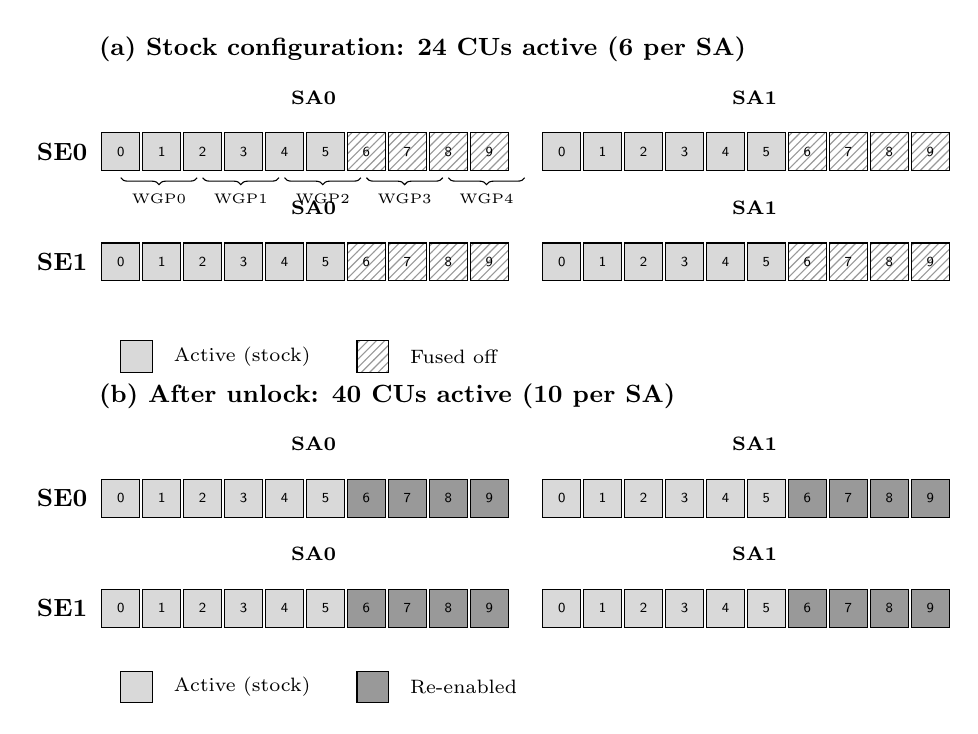
\begin{tikzpicture}[
    cu/.style={minimum width=0.48cm, minimum height=0.48cm, draw=black, font=\tiny\sffamily, inner sep=0pt, line width=0.4pt},
    active/.style={cu, fill=black!15},
    fused/.style={cu, fill=white, pattern=north east lines, pattern color=black!40},
    unlocked/.style={cu, fill=black!40},
    salabel/.style={font=\scriptsize\bfseries, anchor=south},
    selabel/.style={font=\small\bfseries},
]

% --- STOCK ---
\node[font=\small\bfseries, anchor=west] at (-0.4, 1.3) {(a) Stock configuration: 24 CUs active (6 per SA)};

\foreach \xoff/\yoff/\salbl in {0/0/SA0, 5.6/0/SA1, 0/-1.4/SA0, 5.6/-1.4/SA1} {
    \begin{scope}[shift={(\xoff,\yoff)}]
    \node[salabel] at (2.45,0.48) {\salbl};
    \foreach \i in {0,...,5} {
        \node[active] at (\i*0.52, 0) {\i};
    }
    \foreach \i in {6,...,9} {
        \node[fused] at (\i*0.52, 0) {\i};
    }
    \end{scope}
}

\node[selabel, anchor=east] at (-0.3, 0) {SE0};
\node[selabel, anchor=east] at (-0.3, -1.4) {SE1};

% WGP brackets on SE0/SA0
\draw[decorate, decoration={brace, amplitude=2.5pt, mirror}]
    (0,-0.33) -- (0.97,-0.33) node[midway, below=2.5pt, font=\tiny] {WGP0};
\draw[decorate, decoration={brace, amplitude=2.5pt, mirror}]
    (1.04,-0.33) -- (2.01,-0.33) node[midway, below=2.5pt, font=\tiny] {WGP1};
\draw[decorate, decoration={brace, amplitude=2.5pt, mirror}]
    (2.08,-0.33) -- (3.05,-0.33) node[midway, below=2.5pt, font=\tiny] {WGP2};
\draw[decorate, decoration={brace, amplitude=2.5pt, mirror}]
    (3.12,-0.33) -- (4.09,-0.33) node[midway, below=2.5pt, font=\tiny] {WGP3};
\draw[decorate, decoration={brace, amplitude=2.5pt, mirror}]
    (4.16,-0.33) -- (5.13,-0.33) node[midway, below=2.5pt, font=\tiny] {WGP4};

% Legend for stock
\node[active, minimum width=0.4cm, minimum height=0.4cm] at (0.2, -2.6) {};
\node[font=\scriptsize, anchor=west] at (0.55, -2.6) {Active (stock)};
\node[fused, minimum width=0.4cm, minimum height=0.4cm] at (3.2, -2.6) {};
\node[font=\scriptsize, anchor=west] at (3.55, -2.6) {Fused off};

% --- UNLOCKED ---
\begin{scope}[shift={(0,-4.4)}]
\node[font=\small\bfseries, anchor=west] at (-0.4, 1.3) {(b) After unlock: 40 CUs active (10 per SA)};

\foreach \xoff/\yoff/\salbl in {0/0/SA0, 5.6/0/SA1, 0/-1.4/SA0, 5.6/-1.4/SA1} {
    \begin{scope}[shift={(\xoff,\yoff)}]
    \node[salabel] at (2.45,0.48) {\salbl};
    \foreach \i in {0,...,5} {
        \node[active] at (\i*0.52, 0) {\i};
    }
    \foreach \i in {6,...,9} {
        \node[unlocked] at (\i*0.52, 0) {\i};
    }
    \end{scope}
}
\node[selabel, anchor=east] at (-0.3, 0) {SE0};
\node[selabel, anchor=east] at (-0.3, -1.4) {SE1};

% Legend for unlocked
\node[active, minimum width=0.4cm, minimum height=0.4cm] at (0.2, -2.4) {};
\node[font=\scriptsize, anchor=west] at (0.55, -2.4) {Active (stock)};
\node[unlocked, minimum width=0.4cm, minimum height=0.4cm] at (3.2, -2.4) {};
\node[font=\scriptsize, anchor=west] at (3.55, -2.4) {Re-enabled};
\end{scope}

\end{tikzpicture}
\caption{BC-250 die topology showing CU harvest pattern across 2~shader engines $\times$ 2~shader arrays. (a)~Stock: CUs~0--5 active, CUs~6--9 fused off per SA (24 total). (b)~After register modification: all 40~CUs active. Pattern is identical across all three boards tested.}
\label{fig:die}
\end{figure*}

\section{Methodology}

\subsection{Approach Evolution}

Direct register access from an external kernel module was attempted first and proved unworkable. The GPU's power management (GFXOFF) and the \texttt{amdgpu} driver's exclusive ownership of indirect register access paths created an inherent race condition. Three separate attempts crashed the board via deadlock with the driver's \texttt{pcie\_idx\_lock}.

We pivoted to patching the \texttt{amdgpu} kernel driver source directly (Linux 6.19.14, Debian), placing all register reads and writes inside the driver's own GFX initialization path where the GRBM bank-selection lock is already held.

\subsection{Baseline Characterization}

We instrumented the driver's per-shader-array WGP bitmap function (\texttt{gfx\_v10\_0\_get\_wgp\_active\_bitmap\-\_per\_sh}) to log raw register state during CU enumeration:

\begin{lstlisting}
SE0 SH0: cc_raw=0xfff80000
         cc_inactive=0x0000fff8
         active_wgp=0x00000007
SE0 SH1: [identical]
SE1 SH0: [identical]
SE1 SH1: [identical]
\end{lstlisting}

The out-of-range mask (\texttt{0xffffffe0}) marks WGP bits 5+ as physically nonexistent. Within the valid 5-WGP range, \texttt{cc\_inactive=0xfff8} disables WGPs~3 and~4 in every shader array on our three boards.

\subsection{Community Harvest Map Survey}

Following publication of the unlock patch, the BC-250 Discord community collected CU harvest maps from 55+ boards using a standardized script authored by Studebaker (Figure~\ref{fig:harvest}). Key findings:

\begin{itemize}[nosep]
    \item \textbf{100\% of boards} have exactly 24/40 CUs active (6 per SA).
    \item \textbf{$\sim$74\%} show the identical contiguous pattern across all 4~SAs: CUs~0--5 active, CUs~6--9 fused.
    \item \textbf{$\sim$26\%} have at least one SA with a non-contiguous harvest pattern.
    \item At least one board with a ``clean'' contiguous map exhibited 3~faulty CU pairs after unlock.
\end{itemize}

The uniform 24-CU count across all boards confirms deliberate SKU binning. The mix of contiguous and non-contiguous patterns suggests AMD applied a fixed 6-CU-per-SA quota but allowed the specific CUs disabled to vary---likely reflecting actual defect locations on some dies while using a default contiguous mask on fully functional dies. The existence of boards with faulty CUs after unlock underscores the importance of compute verification (Section~4.3).

\begin{figure}[H]
\centering
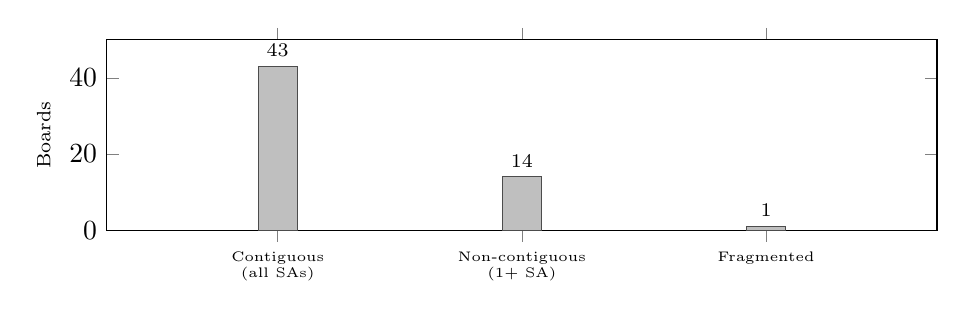
\begin{tikzpicture}
\begin{axis}[
    ybar,
    bar width=14pt,
    width=\columnwidth,
    height=4cm,
    ylabel={Boards},
    ylabel style={font=\scriptsize},
    symbolic x coords={Contiguous\\(all SAs),Non-contiguous\\(1+ SA),Fragmented},
    xtick=data,
    x tick label style={align=center, font=\tiny},
    ymin=0,
    ymax=50,
    nodes near coords,
    nodes near coords style={font=\scriptsize\bfseries},
    enlarge x limits=0.35,
    cycle list={{fill=black!25, draw=black!70}},
]
\addplot[fill=black!25, draw=black!70] coordinates {
    ({Contiguous\\(all SAs)}, 43)
    ({Non-contiguous\\(1+ SA)}, 14)
    ({Fragmented}, 1)
};
\end{axis}
\end{tikzpicture}
\caption{Harvest pattern distribution across 58 community-reported boards. Most show the standard contiguous pattern; a minority have non-contiguous harvesting in one or more shader arrays, likely reflecting genuine defect locations.}
\label{fig:harvest}
\end{figure}

\subsection{Write-Probe Experiment}

We added a guarded boot parameter (\texttt{bc250\_cc\_write\_mode}) to the patched driver with multiple modes:

\begin{itemize}[nosep]
    \item \textbf{Mode 0}: No modification (baseline).
    \item \textbf{Mode 1}: Write zero, read back, restore.
    \item \textbf{Mode 2}: Clear SE0/SH0, no restore.
    \item \textbf{Mode 3}: Clear all 4~SAs, no restore.
    \item \textbf{Mode 4}: Write/read/restore all 4~SAs.
\end{itemize}

Mode~1 (write-then-restore on SE0/SH0) yielded:

\begin{lstlisting}
original     = 0xfff80000
after_zero   = 0xffe00000
after_restore= 0xfff80000
\end{lstlisting}

The upper out-of-range bits remained set, but the valid inactive-WGP bits cleared. This proved that \texttt{CC\_GC\_SHADER\_ARRAY\_CONFIG} is \textbf{not} a read-only hardware fuse latch on this silicon.

\subsection{Boot Safety Mechanism}

To prevent a failed CU-enable from persisting across reboots, we used a self-deleting one-shot modprobe rule:

\begin{lstlisting}
install amdgpu /bin/sh -c \
  'rm -f /etc/modprobe.d/bc250-cc-\
   oneshot.conf; \
   exec /sbin/modprobe --ignore-install \
   amdgpu bc250_cc_write_mode=3'
\end{lstlisting}

The rule removes itself before invoking the driver, ensuring that a crash during the enable attempt does not loop on subsequent power cycles.

\subsection{Discovery of the Second Register}

Initial mode-3 boots produced 40-CU enumeration and correct Vulkan compute results, but LLM inference throughput showed no improvement. Investigation using AMD's UMR (User-Mode Register debugger) revealed a second gate: \texttt{SPI\_PG\_ENABLE\_STATIC\_WGP\_MASK} (offset \texttt{0x1277}).

At stock, this register is \texttt{0x7}---enabling hardware dispatch only to WGPs~0--2. Even with the CC mask cleared, the shader processor continued routing work to only the original 3~WGPs. Setting this register to \texttt{0x1F} via UMR at runtime, combined with the CC clear at boot, unlocked actual compute scaling.

A companion register, \texttt{RLC\_PG\_ALWAYS\_ON\_WGP\_MASK}, must also be set to \texttt{0x1F} to prevent the Run List Controller from power-gating re-enabled WGPs during idle periods. Figure~\ref{fig:gating} illustrates the dual-register gating architecture.

\begin{figure}[H]
\centering
\resizebox{\columnwidth}{!}{%
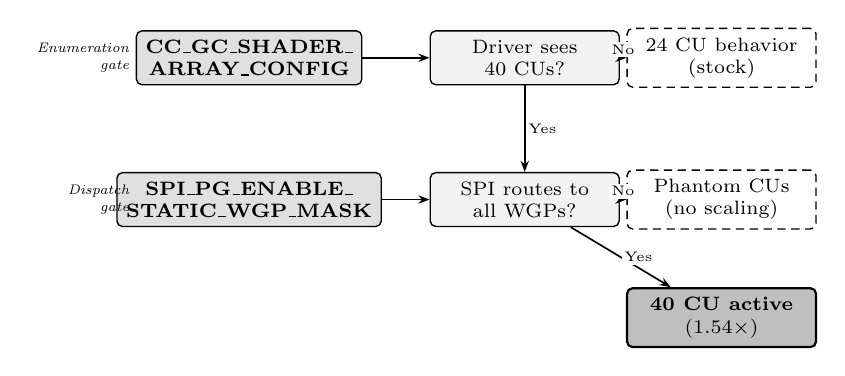
\begin{tikzpicture}[
    box/.style={draw=black, rounded corners=2pt, minimum width=2.4cm, minimum height=0.6cm, align=center, font=\scriptsize, line width=0.5pt},
    regbox/.style={box, fill=black!12},
    state/.style={box, fill=black!5},
    result/.style={box, fill=black!25, line width=0.8pt},
    noresult/.style={box, fill=white, densely dashed},
    arr/.style={-{Stealth[length=4pt]}, semithick},
    lbl/.style={font=\tiny, fill=white, inner sep=1pt},
]

\node[regbox] (cc) at (0, 0) {\textbf{CC\_GC\_SHADER\_}\\\textbf{ARRAY\_CONFIG}};
\node[regbox] (spi) at (0, -1.8) {\textbf{SPI\_PG\_ENABLE\_}\\\textbf{STATIC\_WGP\_MASK}};

\node[font=\tiny\itshape, anchor=east, align=right] at (-1.4, 0) {Enumeration\\gate};
\node[font=\tiny\itshape, anchor=east, align=right] at (-1.4, -1.8) {Dispatch\\gate};

\node[state] (d1) at (3.5, 0) {Driver sees\\40 CUs?};
\node[state] (d2) at (3.5, -1.8) {SPI routes to\\all WGPs?};

\node[noresult] (no1) at (6.0, 0) {24 CU behavior\\(stock)};
\node[noresult] (no2) at (6.0, -1.8) {Phantom CUs\\(no scaling)};
\node[result] (yes) at (6.0, -3.3) {\textbf{40 CU active}\\(1.54$\times$)};

\draw[arr] (cc) -- (d1);
\draw[arr] (d1) -- node[lbl, above] {No} (no1);
\draw[arr] (d1) -- node[lbl, right] {Yes} (d2);
\draw[arr] (d2) -- node[lbl, above] {No} (no2);
\draw[arr] (d2) -- node[lbl, right] {Yes} (yes);
\draw[arr] (spi) -- (d2);

\end{tikzpicture}%
}
\caption{Dual-register gating architecture. Both the CC enumeration mask and SPI dispatch mask must be set; either alone produces no performance change.}
\label{fig:gating}
\end{figure}

\section{Results}

\subsection{4-State Controlled Experiment}

Table~\ref{tab:4state} presents the controlled experiment isolating each register's contribution, measured via 512-token LLM prefill at 2~GHz on bc250-2.

\begin{table}[H]
\centering
\caption{4-state A/B test: register contributions.}
\label{tab:4state}
\small
\begin{tabular}{@{}ccccl@{}}
\toprule
\textbf{CC} & \textbf{SPI} & \textbf{tok/s} & \textbf{W} & \textbf{Scale} \\
\midrule
Stock & 0x7 & 302 & 56 & 1.00$\times$ \\
Stock & 0x1F & 302 & 56 & 1.00$\times$ \\
Clear & 0x7 & 302 & 56 & 1.00$\times$ \\
Clear & 0x1F & \textbf{466} & \textbf{181} & \textbf{1.54$\times$} \\
\bottomrule
\end{tabular}
\end{table}

Neither register alone produces any gain. Both must be set: \texttt{CC\_GC\_SHADER\_ARRAY\_CONFIG} controls CU \textit{enumeration} (driver visibility), while \texttt{SPI\_PG\_ENABLE\_STATIC\_WGP\_MASK} controls hardware \textit{dispatch} (physical wavefront routing).

\subsection{Operating Point Optimization}

At 2~GHz, the 40-CU configuration draws 181W and approaches thermal limits. Table~\ref{tab:oppoint} shows the sustainable 1500~MHz / 900~mV point.

\begin{table}[H]
\centering
\caption{24-CU vs 40-CU at 1500~MHz.}
\label{tab:oppoint}
\small
\begin{tabular}{@{}lcccc@{}}
\toprule
\textbf{Config} & \textbf{tok/s} & \textbf{W} & \textbf{$^\circ$C} & \textbf{Scale} \\
\midrule
24 CU @ 1500 & 230 & 55 & 71 & 1.00$\times$ \\
40 CU @ 1500 & 372 & 125 & 83 & \textbf{1.61$\times$} \\
\bottomrule
\end{tabular}
\end{table}

The 1.61$\times$ scaling at 1500~MHz exceeds the 1.54$\times$ at 2~GHz because the lower clock avoids power limiters, allowing better utilization of the wider shader array. GPU frequency management is handled by the community-developed \texttt{cyan-skillfish-governor-smu} (Section~\ref{sec:community}). Figure~\ref{fig:perf} summarizes the performance results.

\begin{figure}[H]
\centering
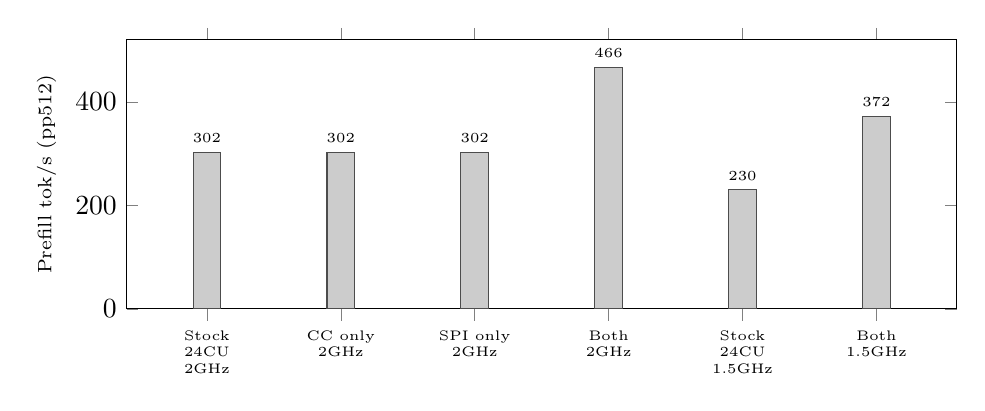
\begin{tikzpicture}
\begin{axis}[
    ybar,
    bar width=10pt,
    width=\columnwidth,
    height=5cm,
    ylabel={Prefill tok/s (pp512)},
    ylabel style={font=\scriptsize},
    symbolic x coords={Stock\\24CU\\2GHz, CC only\\2GHz, SPI only\\2GHz, Both\\2GHz, Stock\\24CU\\1.5GHz, Both\\1.5GHz},
    xtick=data,
    x tick label style={align=center, font=\tiny},
    ymin=0,
    ymax=520,
    nodes near coords,
    nodes near coords style={font=\tiny\bfseries},
    enlarge x limits=0.12,
    cycle list={{fill=black!20, draw=black!70}},
]
\addplot[fill=black!20, draw=black!70] coordinates {
    ({Stock\\24CU\\2GHz}, 302)
    ({CC only\\2GHz}, 302)
    ({SPI only\\2GHz}, 302)
    ({Both\\2GHz}, 466)
    ({Stock\\24CU\\1.5GHz}, 230)
    ({Both\\1.5GHz}, 372)
};
\end{axis}
\end{tikzpicture}
\caption{LLM prefill throughput across all tested configurations. Only the combined CC+SPI modification produces a gain. The 1.5~GHz point achieves better scaling (1.61$\times$) than 2~GHz (1.54$\times$) due to reduced power limiting.}
\label{fig:perf}
\end{figure}

\subsection{Compute Correctness}

Vulkan compute verification was performed at each state:

\begin{itemize}[nosep]
    \item \textbf{28-CU} (1~SA cleared): 1M and 4M element Vulkan shader dispatch, zero errors.
    \item \textbf{40-CU} (all SAs cleared): 1M and 4M element dispatch, zero errors.
    \item \textbf{Stress}: 10 consecutive 4M-element runs at 40~CUs---zero errors, zero GPU recovery events, zero ring timeouts, zero VM faults.
\end{itemize}

No \texttt{amdgpu} reset or fault messages appeared in kernel logs during any test. GPU temperature during sustained 40-CU stress: 70--71$^\circ$C at 1500~MHz.

\subsection{Reproducibility Across Boards}

The enable procedure was validated across multiple boot cycles on three physically separate boards:

\begin{enumerate}[nosep]
    \item Boot to baseline 24~CUs (verified via RADV).
    \item Install one-shot modprobe config, reboot.
    \item Verify 40~CUs: all SAs report \texttt{cu\_mask\,=\,0x3ff}.
    \item Set SPI dispatch mask via UMR.
    \item Run workload, verify scaling.
    \item Reboot---returns to baseline 24~CUs.
\end{enumerate}

All three boards (bc250-1, bc250-2, bc250-3) showed identical behavior and identical harvest patterns. The boards were independently sourced at different times and showed no variation in the CC mask, SPI mask, or CU layout.

\subsection{Cluster Deployment}

Following single-board validation, all three boards were deployed as a Vulkan RPC inference cluster, each running at 40~CUs. The cluster runs a 22~GB Qwen3.6 35B-A3B MoE model split across boards, achieving 187~tok/s prefill and 28~tok/s generation at 128-token context, with 32K context achievable using Q4\_0 KV cache quantization. The boards boot disklessly via PXE/iSCSI from a NAS appliance.

\section{Discussion}

\subsection{Why Are These CUs Functional?}

The community harvest map survey (Section~3.3, $n=58$) reveals a nuanced picture. Approximately 74\% of boards show a perfectly contiguous pattern across all 4~SAs, consistent with a deliberate SKU mask applied to fully functional silicon. The remaining 26\% show at least one SA with a non-contiguous pattern, suggesting genuine defect-driven harvesting on those dies.

All boards share the same 24/40 CU quota, confirming a fixed SKU definition. The BC-250 uses Navi~10 dies that failed PS5 qualification (which requires 36/40~CUs). AMD appears to have applied a uniform 6-CU-per-SA quota, using a default contiguous mask on defect-free dies and mapping actual defect locations on others.

On our three boards (all contiguous-pattern), re-enabled CUs compute correctly and survive stress testing. However, at least one community member with a contiguous map reported 3~faulty CU pairs after unlock---demonstrating that the harvest map alone is not a reliable predictor of CU health, and compute verification is essential.

\subsection{Dual-Register Gating Architecture}

The two-register mechanism provides defense in depth:

\begin{enumerate}[nosep]
    \item \textbf{CC\_GC\_SHADER\_ARRAY\_CONFIG} controls CU \textit{enumeration}. When WGPs are marked inactive, the driver reports fewer CUs and the runtime allocates work accordingly.
    \item \textbf{SPI\_PG\_ENABLE\_STATIC\_WGP\_MASK} controls hardware \textit{dispatch}. Even if the driver sees 40~CUs, the shader processor only routes wavefronts to WGPs enabled here.
\end{enumerate}

Clearing only the enumeration mask creates a ``phantom CU'' state---the driver believes additional CUs exist, but work is silently routed to the enabled subset. This produces no errors and no performance change.

\subsection{Economics of Salvage Compute}

Table~\ref{tab:economics} compares the per-CU economics at current secondary market prices (\$50--150).

\begin{table}[H]
\centering
\caption{Economics: stock vs.\ unlocked BC-250 (at \$150).}
\label{tab:economics}
\small
\begin{tabular}{@{}lcc@{}}
\toprule
\textbf{Metric} & \textbf{24 CU} & \textbf{40 CU} \\
\midrule
pp512 @ 1500 MHz & 230 tok/s & 372 tok/s \\
\$/CU & \$6.25 & \$3.75 \\
Perf/\$ (tok/s/\$) & 1.53 & 2.48 \\
tok/s/W & 4.18 & 2.98 \\
\bottomrule
\end{tabular}
\end{table}

At the low end of the price range (\$50), the unlocked 40-CU configuration delivers 7.44~tok/s/\$---competitive with consumer GPUs costing an order of magnitude more, provided the workload fits in 16~GB of unified memory.

\subsection{Broader Applicability}

The methodology---instrumenting the driver's own init path to test register writability under proper locking---is applicable to other AMD products. Whether other harvested parts (e.g., RX~7800~XT vs RX~7900~XTX) use similarly writable CC masks is an open question. The gfx1013 variant's origin as a repurposed console APU may make it uniquely permissive.

\subsection{Limitations}

\begin{itemize}[nosep]
    \item \textbf{Persistence}: The CC mask reverts on reboot; the SPI mask must be set post-boot. A production deployment should integrate both writes into the driver init path.
    \item \textbf{CPU cores}: The APU's CPU harvesting (6/8 Zen~2 cores) is PSP-enforced and not clearable via this technique. INIT/SIPI signals to disabled cores return error status 0x4.
    \item \textbf{Thermal ceiling}: 40~CUs at 2~GHz draw 181W. The 1500~MHz / 900~mV point (125W) is recommended for sustained workloads.
    \item \textbf{Sample size}: Three boards tested with identical results. Population-level confidence requires broader community replication.
    \item \textbf{Defect risk}: Some boards may carry genuinely defective CUs. Extended compute verification is essential before relying on re-enabled CUs.
\end{itemize}

\section{Community Ecosystem}
\label{sec:community}

This work builds on a substantial open-source ecosystem developed by the BC-250 community (3,500+ members on Discord). While the CU re-enablement technique is novel, the platform's viability as a compute node depends on prior community contributions:

\textbf{Custom BIOS firmware.}
TuxThePenguin0 (``Segfault'') developed modified BIOS images that unlock dynamic VRAM allocation and chipset configuration menus, enabling the flexible memory split between CPU and GPU that makes inference workloads practical on a 16~GB unified memory system~\cite{bios}.

\textbf{GPU power management.}
FilippoR's \texttt{cyan-skillfish-governor-smu}~\cite{governor_smu} provides SMU-based GPU clock/voltage scaling. Without a governor, the BC-250 GPU locks at 1500~MHz regardless of load. The governor enables the variable clock states used in our operating-point analysis. mothenjoyer69's earlier \texttt{oberon-governor}~\cite{governor} established the initial approach.

\textbf{CPU overclocking and ACPI.}
The bc250-collective's \texttt{bc250\_smu\_oc} tool enables Zen~2 CPU frequency adjustment via SMU mailbox. Their \texttt{bc250-acpi-fix} provides SSDT tables for proper C-State and P-State enumeration~\cite{smuoc,acpifix}.

\textbf{Kernel contributions.}
Magnap identified the critical TTM page limit fix (\texttt{ttm.pages\_limit=4194304}) that unlocks full 16~GB memory allocation; without this parameter, the GPU is capped at $\sim$7.4~GiB.

\textbf{Documentation.}
elektricM compiled comprehensive documentation from over 9,700 Discord messages~\cite{elektric}. mothenjoyer69 authored the original hardware documentation~\cite{mothen}. akandr developed and published inference benchmarks across 31 models, establishing the BC-250's performance envelope~\cite{akandr}.

\textbf{Hardware ecosystem.}
provod developed a ray tracing compatibility patch. Fred78290 authored the \texttt{nct6687d} kernel module~\cite{nct6687d} for fan/thermal control via the Nuvoton NCT6686D SuperIO. Over 145 3D-printable case designs exist on community repositories.

\textbf{Community replication.}
Following publication of the unlock patch, 58 community members submitted CU harvest maps (Section~3.3), and multiple users have successfully applied the unlock procedure to their boards. At least one user reported faulty CU pairs after unlock, confirming that compute verification is essential.

\section{Conclusion}

We demonstrated that the AMD BC-250 APU's GPU CU harvesting is enforced by two software-writable configuration registers rather than irreversible hardware fuses. By clearing \texttt{CC\_GC\_SHADER\_ARRAY\_CONFIG} during kernel driver initialization and setting \texttt{SPI\_PG\_ENABLE\_STATIC\_WGP\_MASK} to enable dispatch to all work-group processors, we re-enabled all 40 physical CUs on a part shipped with 24---a 67\% increase in GPU compute resources from a purely software modification.

The re-enabled CUs are fully functional: they produce correct results, survive sustained stress testing, and deliver 1.54--1.61$\times$ throughput improvement on LLM inference workloads. The technique is reproducible across boot cycles and across three separate boards now operating as a production inference cluster.

This finding challenges the assumption that semiconductor harvesting always represents a permanent physical constraint. For the growing community repurposing salvaged silicon for AI inference, it demonstrates that register-level analysis of hardware gating mechanisms can recover significant compute left on the table by the original manufacturer.

\onecolumn

\section*{Acknowledgments}

This work was conducted as independent research with hardware purchased at secondary market prices. The kernel driver patch and enable tooling are published at \url{https://github.com/duggasco/bc250-40cu-unlock}. AMD's open-source \texttt{amdgpu} kernel driver and Mesa/RADV Vulkan driver made this work possible---the ability to read, instrument, and modify the driver source was the key enabler.

Special thanks to the community contributors whose work made the BC-250 a viable compute platform: TuxThePenguin0 for custom BIOS development~\cite{bios}, FilippoR for the \texttt{cyan-skillfish-governor-smu}~\cite{governor_smu}, mothenjoyer69 for hardware documentation and the original GPU governor~\cite{mothen,governor}, elektricM for compiling community knowledge from over 9,700 Discord messages~\cite{elektric}, akandr for publishing inference benchmarks across 31 models~\cite{akandr}, Magnap for the critical TTM page limit kernel fix, the bc250-collective for SMU overclocking and ACPI tooling~\cite{smuoc,acpifix}, Fred78290 for the fan control kernel module~\cite{nct6687d}, and the 58 Discord community members (\texttt{discord.gg/8eZfFWhczz}) who submitted CU harvest maps for the population survey.

\begin{thebibliography}{10}

\bibitem{unlock}
S.~Duggan, ``BC-250 40-CU Unlock,''
\url{https://github.com/duggasco/bc250-40cu-unlock}, 2026.

\bibitem{bios}
TuxThePenguin0, ``BC-250 Modified BIOS,''
\url{https://gitlab.com/TuxThePenguin0/bc250-bios/}, 2025.

\bibitem{governor_smu}
FilippoR, ``Cyan Skillfish Governor (SMU),''
\url{https://github.com/filippor/cyan-skillfish-governor}, 2025.

\bibitem{governor}
mothenjoyer69, ``Oberon Governor,''
\url{https://gitlab.com/mothenjoyer69/oberon-governor}, 2025.

\bibitem{smuoc}
bc250-collective, ``BC-250 SMU Overclock,''
\url{https://github.com/bc250-collective/bc250_smu_oc}, 2025.

\bibitem{acpifix}
bc250-collective, ``BC-250 ACPI Fix,''
\url{https://github.com/bc250-collective/bc250-acpi-fix}, 2025.

\bibitem{nct6687d}
Fred78290, ``NCT6687D Kernel Module,''
\url{https://github.com/Fred78290/nct6687d}, 2025.

\bibitem{elektric}
elektricM, ``AMD BC-250 Documentation,''
\url{https://github.com/elektricM/amd-bc250-docs}, 2025.

\bibitem{mothen}
mothenjoyer69, ``BC-250 Documentation,''
\url{https://github.com/mothenjoyer69/bc250-documentation}, 2024.

\bibitem{akandr}
akandr, ``BC-250 Inference Benchmarks,''
\url{https://github.com/akandr/bc250}, 2026.

\end{thebibliography}

\appendix

\section{Register Details}

\subsection*{CC\_GC\_SHADER\_ARRAY\_CONFIG}

DWORD offset \texttt{0x2042C}, per-instance \texttt{0x0226f}.

\begin{table}[H]
\centering
\begin{tabular}{@{}llll@{}}
\toprule
\textbf{Bits} & \textbf{Field} & \textbf{Stock} & \textbf{Cleared} \\
\midrule
31:20 & Out-of-range WGP mask & 0xFFE & 0xFFE \\
19:16 & Inactive WGPs (valid) & 0xF (WGP 3--4 off) & 0x0 (all active) \\
15:0 & Reserved & 0x0000 & 0x0000 \\
\bottomrule
\end{tabular}
\end{table}

Full raw value: \texttt{0xFFF80000} (stock) $\rightarrow$ \texttt{0xFFE00000} (cleared).

\subsection*{SPI\_PG\_ENABLE\_STATIC\_WGP\_MASK}

Offset \texttt{0x1277}. Each bit enables hardware shader dispatch to one WGP within each shader array.

\begin{table}[H]
\centering
\begin{tabular}{@{}cclcc@{}}
\toprule
\textbf{Bit} & \textbf{WGP} & \textbf{CUs} & \textbf{Stock} & \textbf{Enabled} \\
\midrule
0 & WGP 0 & CU 0--1 & 1 & 1 \\
1 & WGP 1 & CU 2--3 & 1 & 1 \\
2 & WGP 2 & CU 4--5 & 1 & 1 \\
3 & WGP 3 & CU 6--7 & 0 & 1 \\
4 & WGP 4 & CU 8--9 & 0 & 1 \\
\bottomrule
\end{tabular}
\end{table}

Stock value: \texttt{0x7} (WGPs 0--2 enabled). Unlocked value: \texttt{0x1F} (all 5 WGPs enabled).

\subsection*{RLC\_PG\_ALWAYS\_ON\_WGP\_MASK}

Must be set to \texttt{0x1F} concurrently with \texttt{SPI\_PG\_ENABLE\_STATIC\_WGP\_MASK} to prevent the Run List Controller from power-gating re-enabled WGPs during idle periods.

\section{Harvest Pattern Visualization}

Per-SA CU layout showing the dominant (74\%) contiguous harvest pattern:

\begin{lstlisting}
CU index:     0   1   2   3   4   5   6   7   8   9
             [*] [*] [*] [*] [*] [*] [ ] [ ] [ ] [ ]
              |--- active (stock) --|  |--- fused ---|
              WGP 0    WGP 1    WGP 2    WGP 3    WGP 4
\end{lstlisting}

Non-contiguous variants observed in $\sim$26\% of boards (examples from community survey):
\begin{lstlisting}
Variant A:   [*] [*] [ ] [ ] [*] [*] [*] [*] [ ] [ ]
Variant B:   [ ] [ ] [*] [*] [*] [*] [*] [*] [ ] [ ]
Variant C:   [*] [*] [*] [*] [ ] [ ] [*] [*] [ ] [ ]
\end{lstlisting}

All variants maintain exactly 6 active CUs (3 active WGPs) per shader array. After re-enablement, all 10 CUs per SA are active and dispatching compute work regardless of the original harvest pattern.

\section{Enable Procedure}

\begin{lstlisting}
# 1. Build patched amdgpu module with bc250_cc_write_mode parameter
#    (see https://github.com/duggasco/bc250-40cu-unlock)

# 2. Install one-shot boot config:
echo 'install amdgpu /bin/sh -c '\''rm -f /etc/modprobe.d/bc250-cc-oneshot.conf; \
  exec /sbin/modprobe --ignore-install amdgpu bc250_cc_write_mode=3'\''' \
  > /etc/modprobe.d/bc250-cc-oneshot.conf

# 3. Reboot

# 4. Set SPI dispatch mask (requires umr):
umr -w cyan_skillfish.gfx1013.mmSPI_PG_ENABLE_STATIC_WGP_MASK 0x1f
umr -w cyan_skillfish.gfx1013.mmRLC_PG_ALWAYS_ON_WGP_MASK 0x1f

# 5. Verify:
RADV_DEBUG=info vulkaninfo 2>&1 | grep cu_mask
# Expected: cu_mask = 0x3ff (all SAs)
\end{lstlisting}

\end{document}
